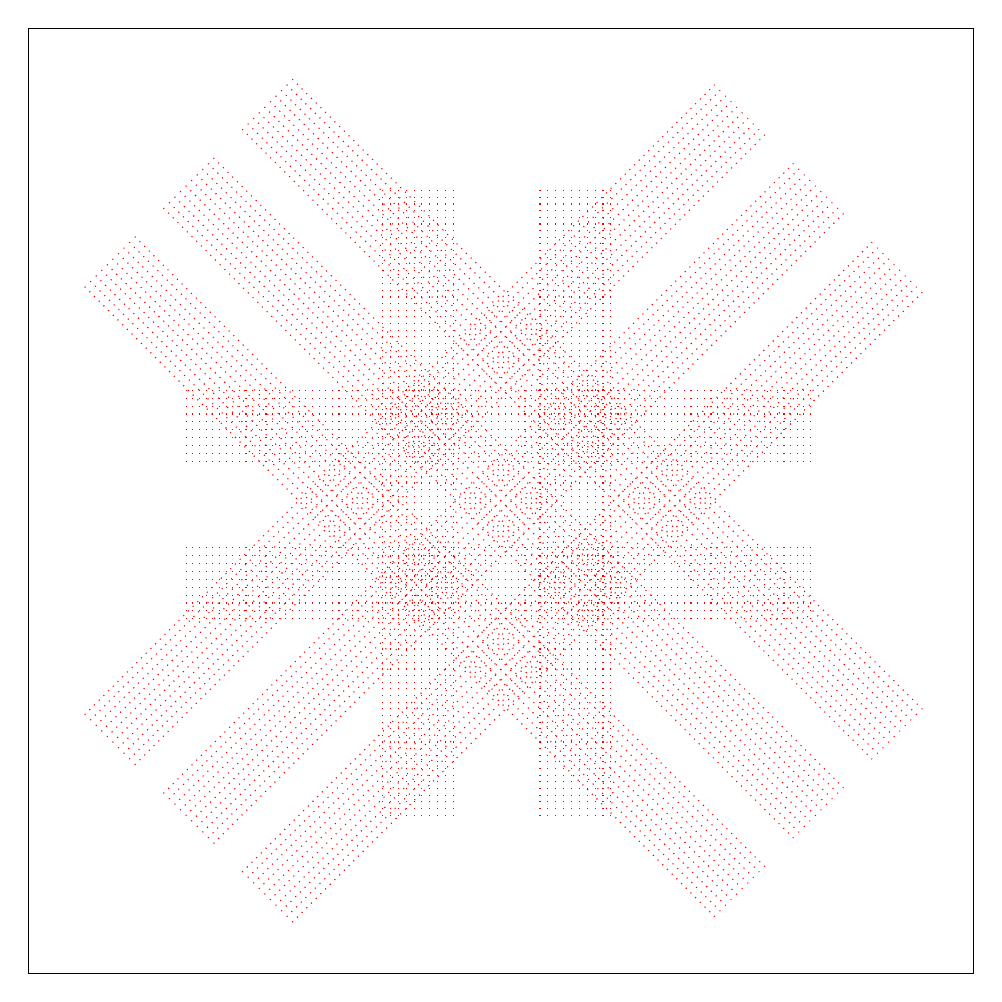
\begin{tikzpicture}
    \draw[black] (-6, -6) -- (-6, 6) -- (6, 6) -- (6, -6) -- cycle;
    \foreach \x in {-0.5, -0.4, ..., 0.5} {
        \draw[dotted, red] ({-1 + \x}, -4) -- ({-1 + \x}, 4);
        \draw[dotted, red] ({1 + \x}, -4) -- ({1 + \x}, 4);

        \draw[dotted, red] (-4, {-1 + \x}) -- (4, {-1 + \x});
        \draw[dotted, red] (-4, {1 + \x}) -- (4, {1 + \x});

        \draw[dotted, red] ({-4 - \x  / sqrt(2)}, {-4 + \x / sqrt(2)}) -- ({4 - \x / sqrt(2)}, {4 + \x / sqrt(2)});
        \draw[dotted, red] ({-4 - (\x+sqrt(2))  / sqrt(2)}, {-4 + (\x+sqrt(2)) / sqrt(2)}) -- ({4 - (\x+sqrt(2)) / sqrt(2)}, {4 + (\x+sqrt(2)) / sqrt(2)});
        \draw[dotted, red] ({-4 - (\x-sqrt(2))  / sqrt(2)}, {-4 + (\x-sqrt(2)) / sqrt(2)}) -- ({4 - (\x-sqrt(2)) / sqrt(2)}, {4 + (\x-sqrt(2)) / sqrt(2)});

        \draw[dotted, red] ({-4 - \x  / sqrt(2)}, {4 - \x / sqrt(2)}) -- ({4 - \x / sqrt(2)}, {-4 - \x / sqrt(2)});
        \draw[dotted, red] ({-4 - (\x+sqrt(2))  / sqrt(2)}, {4 - (\x+sqrt(2)) / sqrt(2)}) -- ({4 - (\x+sqrt(2)) / sqrt(2)}, {-4 - (\x+sqrt(2)) / sqrt(2)});
        \draw[dotted, red] ({-4 - (\x-sqrt(2))  / sqrt(2)}, {4 - (\x-sqrt(2)) / sqrt(2)}) -- ({4 - (\x-sqrt(2)) / sqrt(2)}, {-4 - (\x-sqrt(2)) / sqrt(2)});
    }
\end{tikzpicture}